\chapter{Prezentarea sistemelor similare}\label{ch:2sistemeSimilare}

	In momentul de față, acest subdomeniu se află la un nivel mare de răspândire. Există o serie de producători care comercializează sisteme ce permit controlul la distanță al temperaturii, însă au o deficență majoră, și anume, prețul ridicat. Voi prezenta mai multe astfel de sisteme, împreună cu detaliile tehnice ale acestora. 	

\section{Torelectric}
	Termostatul produs de firma Torelectric oferă mai multe modalități de reglare a temperaturii:
	\begin{itemize}
  	\setlength{\itemindent}{2em}
		\item Prin aplicație mobilă
		\item Fizic, utilizând interfața termostatului
		\item Prin comenzi vocale, utilizând Google Home și Alexa
	\end{itemize}
	

	\begin{figure}[H]
    		\centering
    	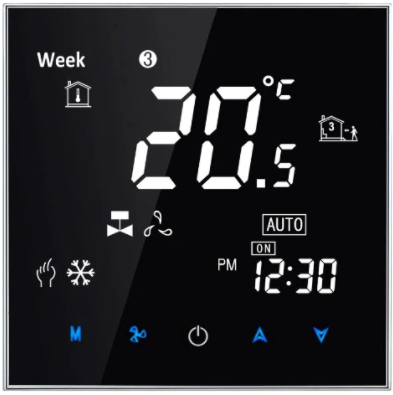
\includegraphics[width=0.4\textwidth]{Torelectric.png}
	\end{figure}

	Ca și caracteristici principale se pot remarca:
	\begin{itemize}
	\setlength{\itemindent}{2em}
		\item Conectivitate: Wi-Fi
		\item Tip alimentare: La retea
		\item Precizie: $\pm 2$ \textdegree{}C sau $\pm 1$ \textdegree{}C
		\item Setare temperatură intre: 5 - 35 \textdegree{}C
		\item Temperatură ambientală: 0 - 45 \textdegree{}C
	\end{itemize}

\begin{wrapfigure}{l}{0.4\textwidth} 
\centering
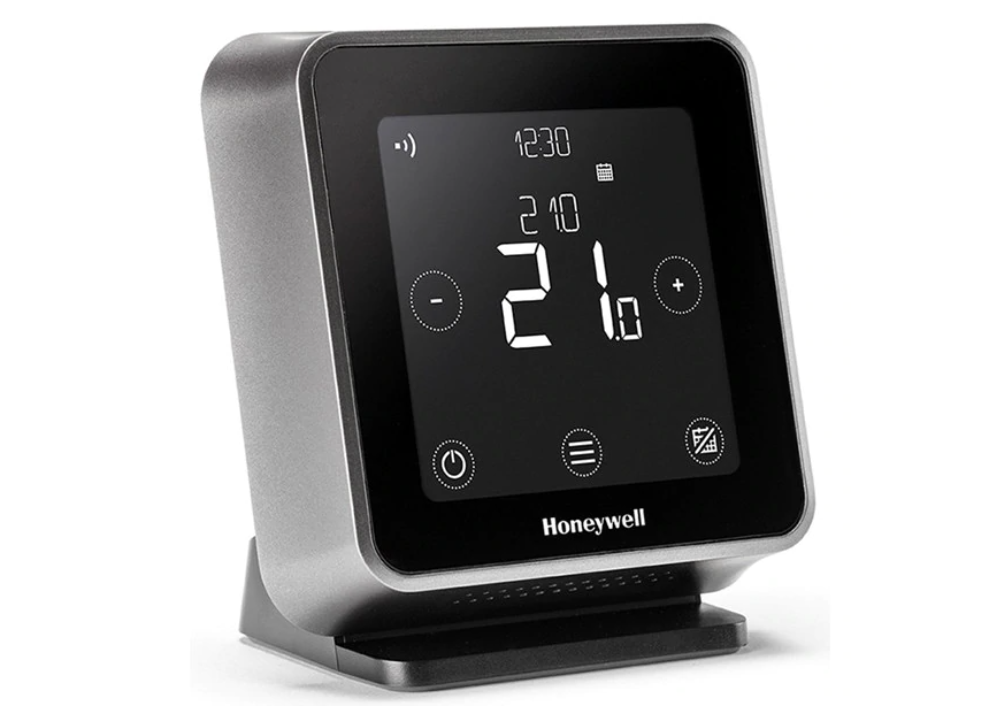
\includegraphics[width=0.4\textwidth]{Honeywell.png}
\end{wrapfigure}
\section{Honeywell}
	Termostatul produs de Honeywell se diferențiază față de cel produs de Torelectric prin prezența unor funcționalități inovatoare. Printre particularitățile acestui dispozitiv se remarcă:
	\begin{itemize}
	\setlength{\itemindent}{2em}
		\item Adaptarea temperaturii în funcție de prezența sau absența unor persoane în locuință 
		\item Programarea temperaturilor pentru șapte zile
		\item Controlul de la distanță, oferit de aplicația mobilă
		\item Setarea temperaturii prin comenzi vocale
	\end{itemize}

	Comparativ cu primul sistem prezentat, cel de la Honeywell se deosebește prin tehnologia Geofencing. Acesta știe când imobilul nu este locuit, iar ca urmare, va dezactiva încălzirea. De asemenea, este capabil să detecteze momentul în care locuitorii sunt în apropierea casei, reușind să încălzească până la temperatura setată.
	Un alt avantaj adus de cei de la Honeywell este posibilitatea de a seta temperatura pe decursul a șapte zile, fapt ce asigură un confort sporit, prin adaptarea temperaturii în funcție de diverse intervale orare.

	Caracteristicile tehnice ale acestuia sunt:
	\begin{itemize}
	\setlength{\itemindent}{2em}
		\item Destinat: centrale termice
		\item Suprafata de montare: masă
		\item Tip alimentare: la rețea
		\item Conectivitate: Wi-Fi
	\end{itemize}

	În continuare, voi prezenta două sisteme care reprezintă apogeul evoluției în acest domeniu. Acestea sunt produse de firme cunoscute precum: Google si Ecobee.

\section{Nest}
	Este un termostat inteligent produs de cei de la Google. Acesta oferă funcționalități avansate pentru un management, cât mai eficient, al temperaturii din imobil. 

	Spre deosebire de sistemele prezentate anterior, termostatele produse de Google Nest integrează tehnologii revoluționare pentru a obține un randament cat mai mare.

\vspace{2em}

	Principalele particularități ale acestuia sunt:
	\begin{itemize}
	\setlength{\itemindent}{2em}
		\item Capacitatea de a se programa automat, în funcție de rutina locuitorilor
		\item Menține temperatura setată doar dacă există persoane în imobil, altfel trece automat la o temperatură ce asigură un consum cât mai mic de energie
		\item Control de la distanță de pe laptop, tabletă și telefon
		\item Salvarea unui istoric al consumului de energie
	\end{itemize}

\vspace{2em}

\begin{wrapfigure}{l}{0.3\textwidth} 
\centering
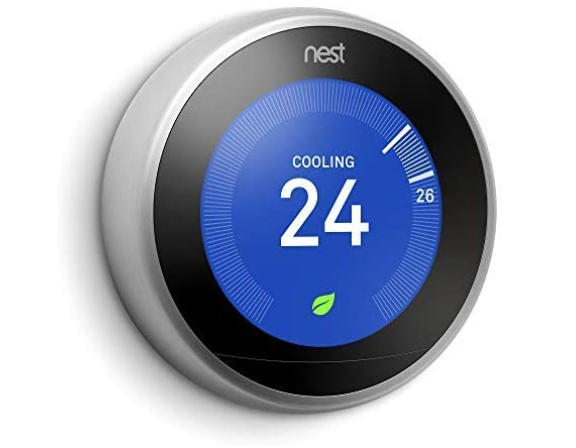
\includegraphics[width=0.3\textwidth]{Nest.png}
\end{wrapfigure}

	Date tehnice:
	\begin{itemize}
	\setlength{\itemindent}{2em}
		\item Sursă de energie: baterii
		\item Tensiune de funcționare: 24 volți
		\item Afișaj digital
		\item Conectivitate: WiFi
	\end{itemize}

\section{Ecobee}
	 Termostatul produs de firma Ecobee poate fi controlat prin intermediul unor aplicații precum: Apple HomeKit, Alexa built-in, Google Assistant, SmartThings. De asemenea, oferă posibilitatea de a seta temperatura de pe Android, dar si de pe iOS.
	
	Acesta implementează un algoritm ce permite controlul temperaturii in diverse locuri din imobil. Se pot conecta mai mulți senzori de temperatura la termostat, iar in funcție de informatiile primite de la aceștia, menține o temperatură constantă în locuință.

	Ecranul se aprinde atunci când detectează o persoană în apropiere, iar pe lângă informațiile legate de temperatură si umiditate, se afișează si vreme pe decursul a cinci zile.

\vspace{2em}

	Date tehnice:
	\begin{itemize}
	\setlength{\itemindent}{2em}
		\item Sursă de energie: baterii
		\item Tensiune de funcționare: 24 volți
		\item Ecran tactil
		\item Conectivitate: WiFi
	\end{itemize}

